\section{Generating Clusters}
 Clusters were generated by sampling from a Gaussian distribution, then transforming the distribution. 
 
 \subsection{Classes A and B}
 The two classes A and B were characterized by:

\begin{eqnarray}
{\mu}_{A}=\left[ \begin{smallmatrix} 5&10 \end{smallmatrix}\right]^{T} \; & {\Sigma}_{A}=\left[ \begin{smallmatrix} 8&0 \\ 0&4 \end{smallmatrix}\right]^{T} \nonumber\\
{\mu}_{B}=\left[ \begin{smallmatrix} 10&15 \end{smallmatrix}\right]^{T} \; & {\Sigma}_{B}=\left[ \begin{smallmatrix} 8&0 \\ 0&4 \end{smallmatrix}\right]^{T} \nonumber
\end{eqnarray}

\begin{figure}[ht]
\centering
	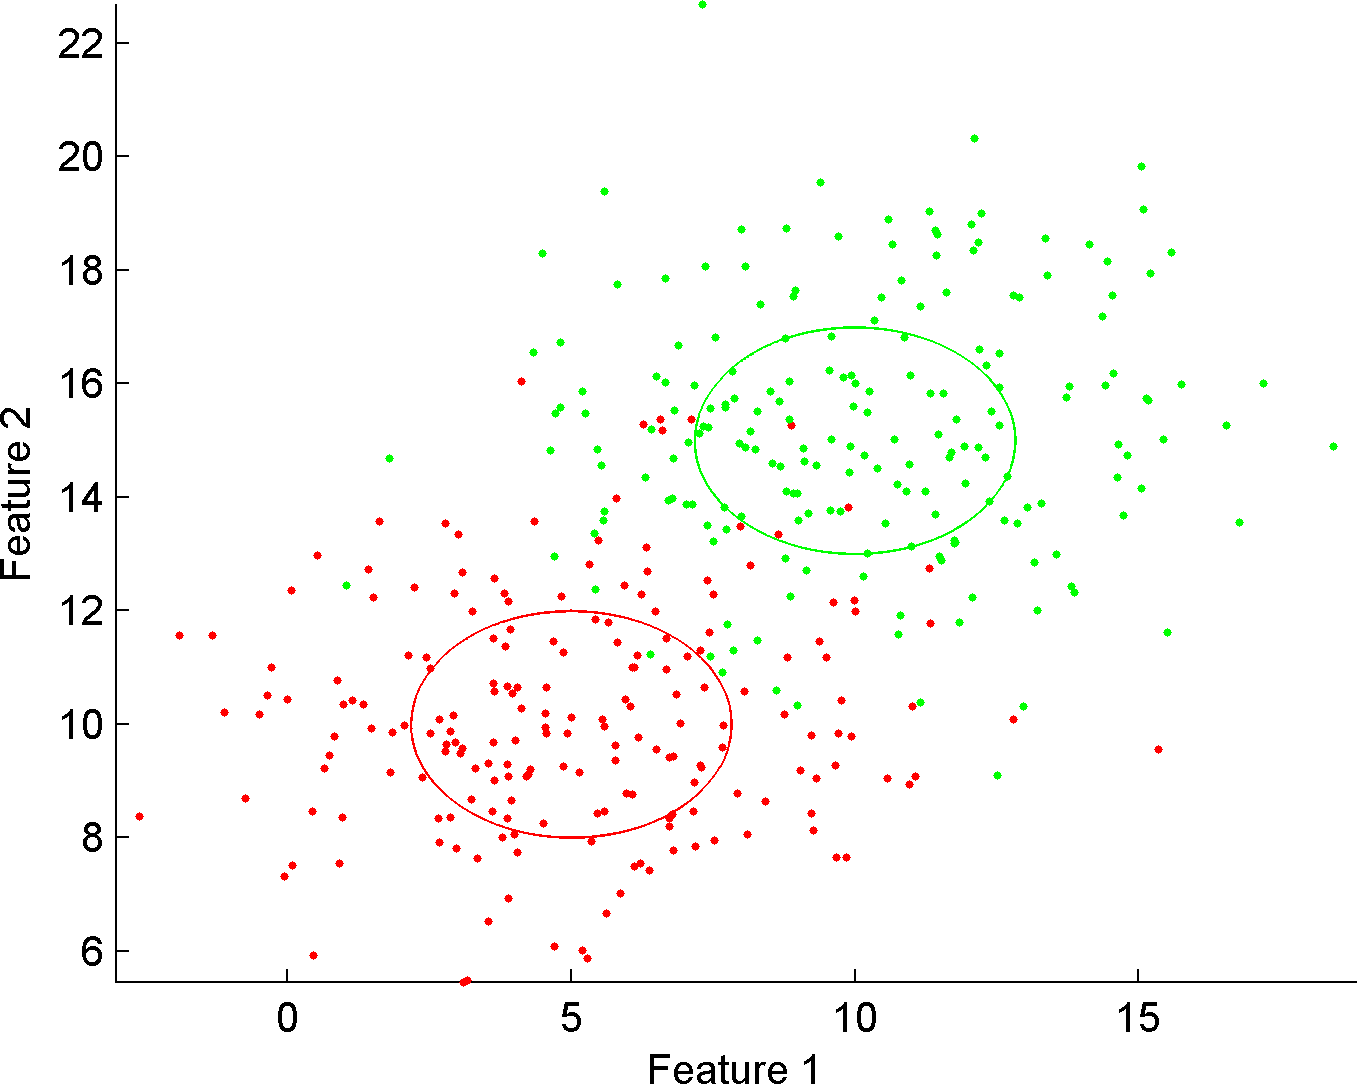
\includegraphics[width=0.9\linewidth]{fig1a-AB_cluster}
	\label{fig:clustersDataAB}
	\caption{Clusters A and B with unit standard deviation elipses}
\end{figure}

 \subsection{Classes C, D, E}
 The three classes C, D and E were characterized by:
 
 \begin{eqnarray}
{\mu}_{C}=\left[ \begin{smallmatrix} 5&10 \end{smallmatrix}\right]^{T} \; & {\Sigma}_{C}=\left[ \begin{smallmatrix} 8&4 \\ 4&40 \end{smallmatrix}\right]^{T} \nonumber\\
{\mu}_{D}=\left[ \begin{smallmatrix} 15&10 \end{smallmatrix}\right]^{T} \; & {\Sigma}_{D}=\left[ \begin{smallmatrix} 8&0 \\ 0&8 \end{smallmatrix}\right]^{T} \nonumber\\
{\mu}_{E}=\left[ \begin{smallmatrix} 10&5 \end{smallmatrix}\right]^{T} \; & {\Sigma}_{D}=\left[ \begin{smallmatrix} 10&-5 \\ -5&20 \end{smallmatrix}\right]^{T} \nonumber
\end{eqnarray}
 
 
\begin{figure}[ht]
\centering
	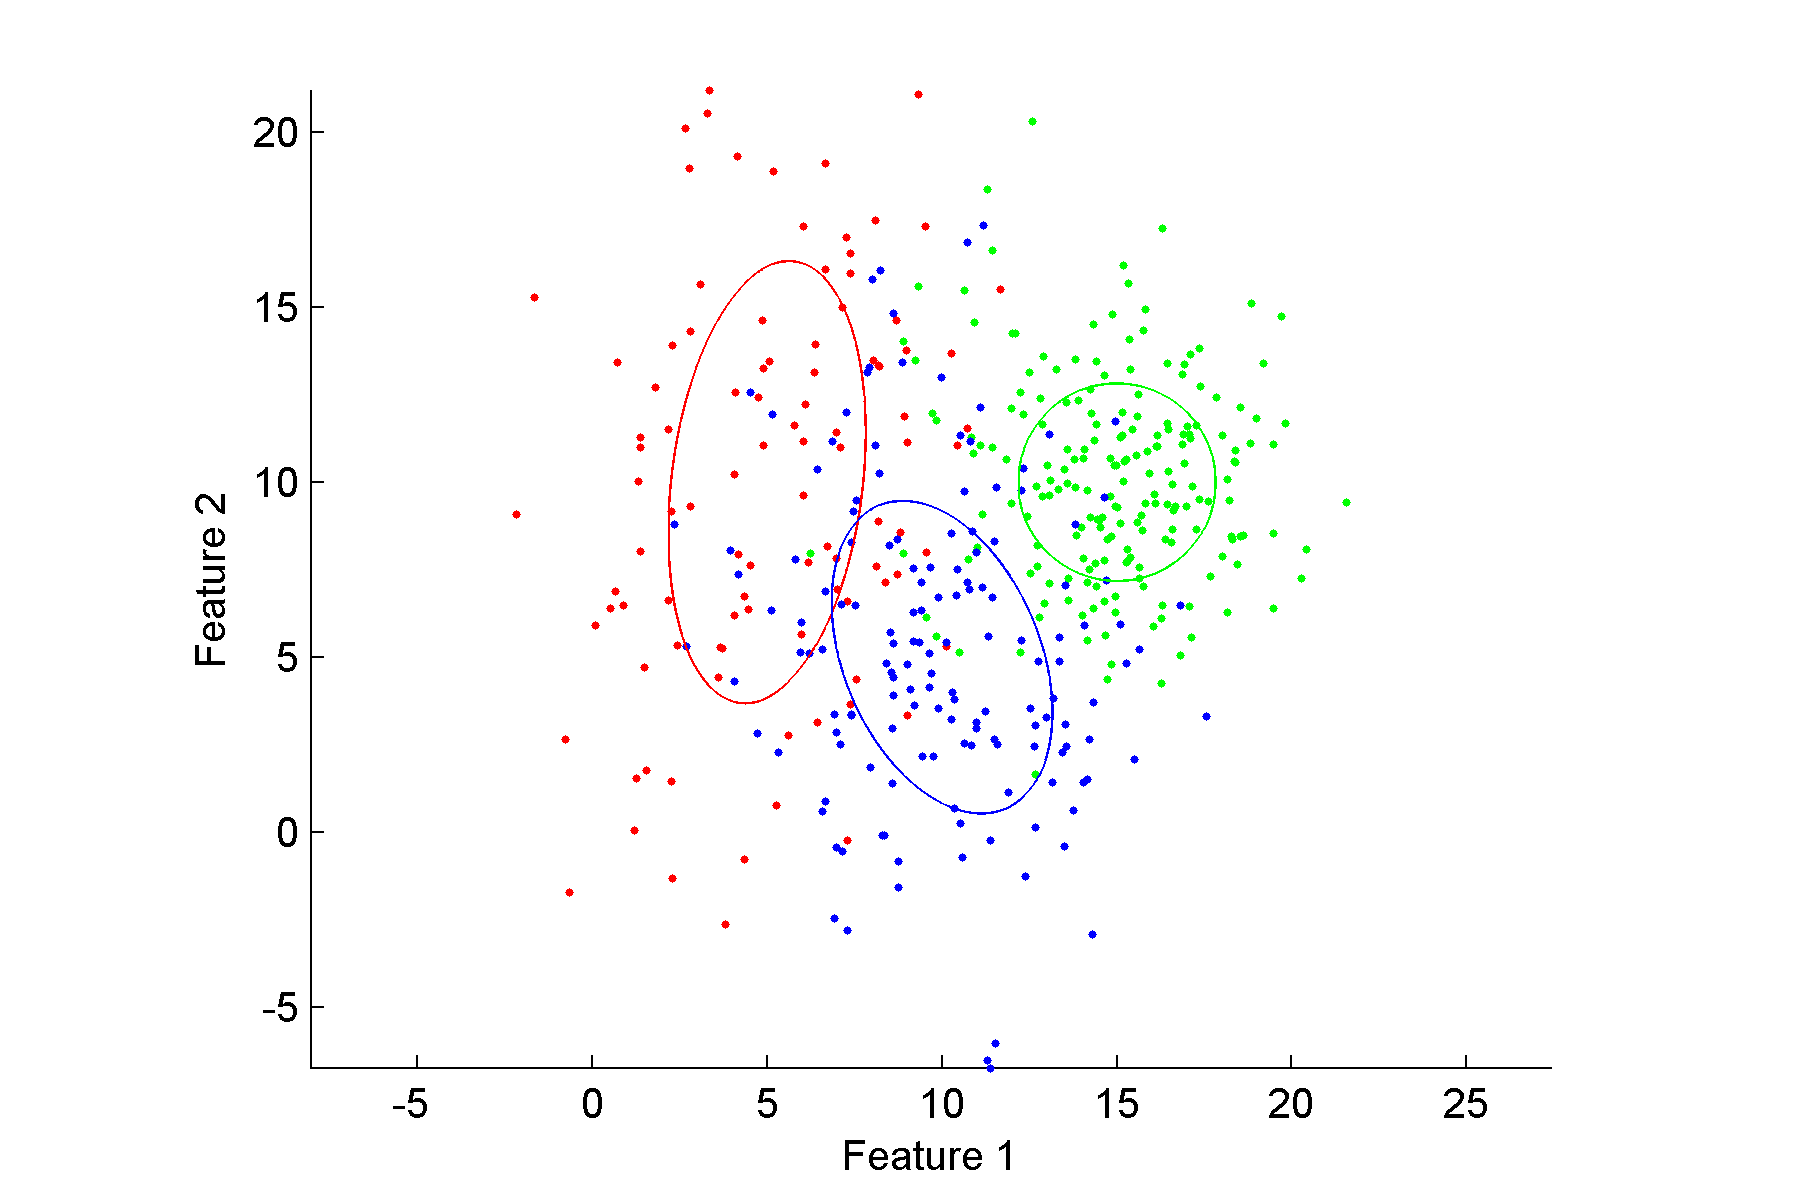
\includegraphics[width=0.9\linewidth]{fig1b-CDE_cluster}
	\label{fig:clustersDataCDE}
	\caption{Clusters C, D, E unit standard deviation elipses}
\end{figure}
 
\clearpage
